\documentclass[12pt]{article}

\usepackage{fullpage}
\usepackage{graphicx, rotating, booktabs} 
\usepackage{times} 
\usepackage{natbib} 
\usepackage{indentfirst} 
\usepackage{setspace}
\usepackage{grffile} 
\usepackage{hyperref}
\usepackage{adjustbox}
\usepackage{amsmath}
\usepackage{siunitx}
\setcitestyle{aysep{}}


\singlespace
\title{\textbf{Appendix: Democracy and Alliance Treaty Depth}}
\author{}
\date{}

\bibliographystyle{apsr}

\begin{document}

\maketitle 

\doublespace 

This appendix contains a series of robustness checks for the findings in the manuscript. 
In the first section, I examine results with an alternative measure of democracy when the alliance formed: the proportion of democracies in the alliance. 
Then I look at results from two altnerative measures of treaty depth.  
Last, I consider how uncertainty in the latent treaty depth measure affects my inferences. 


\section{Proportion of Democracies}


In the paper, I use the average polity score of all alliance members when the treaty as the key independent variable. 
The proportion of democracies in the alliance is an alternative measure of how much heft democracies have in negotiations \cite{Chibaetal2015}.  
Rather than average the POLITY scores of alliance members, this variable is the share of alliance members with a POLITY score greater than 5, which is a common threshold for democracy. 
My argument anticipates that the proportion measure should lead to similar inferences about the connection between democracy and alliance treaty depth.


First, the descriptive statistics for the proportion of democracies across treaty depth and unconditional military support are as expected. 
\autoref{fig:democ-prop-combo} shows the average proportion of democracies in four types of alliances. 
Deep, conditional alliances have the highest average proportion of democratic members, although it is not much higher than the shallow and conditional average.  


\begin{figure}
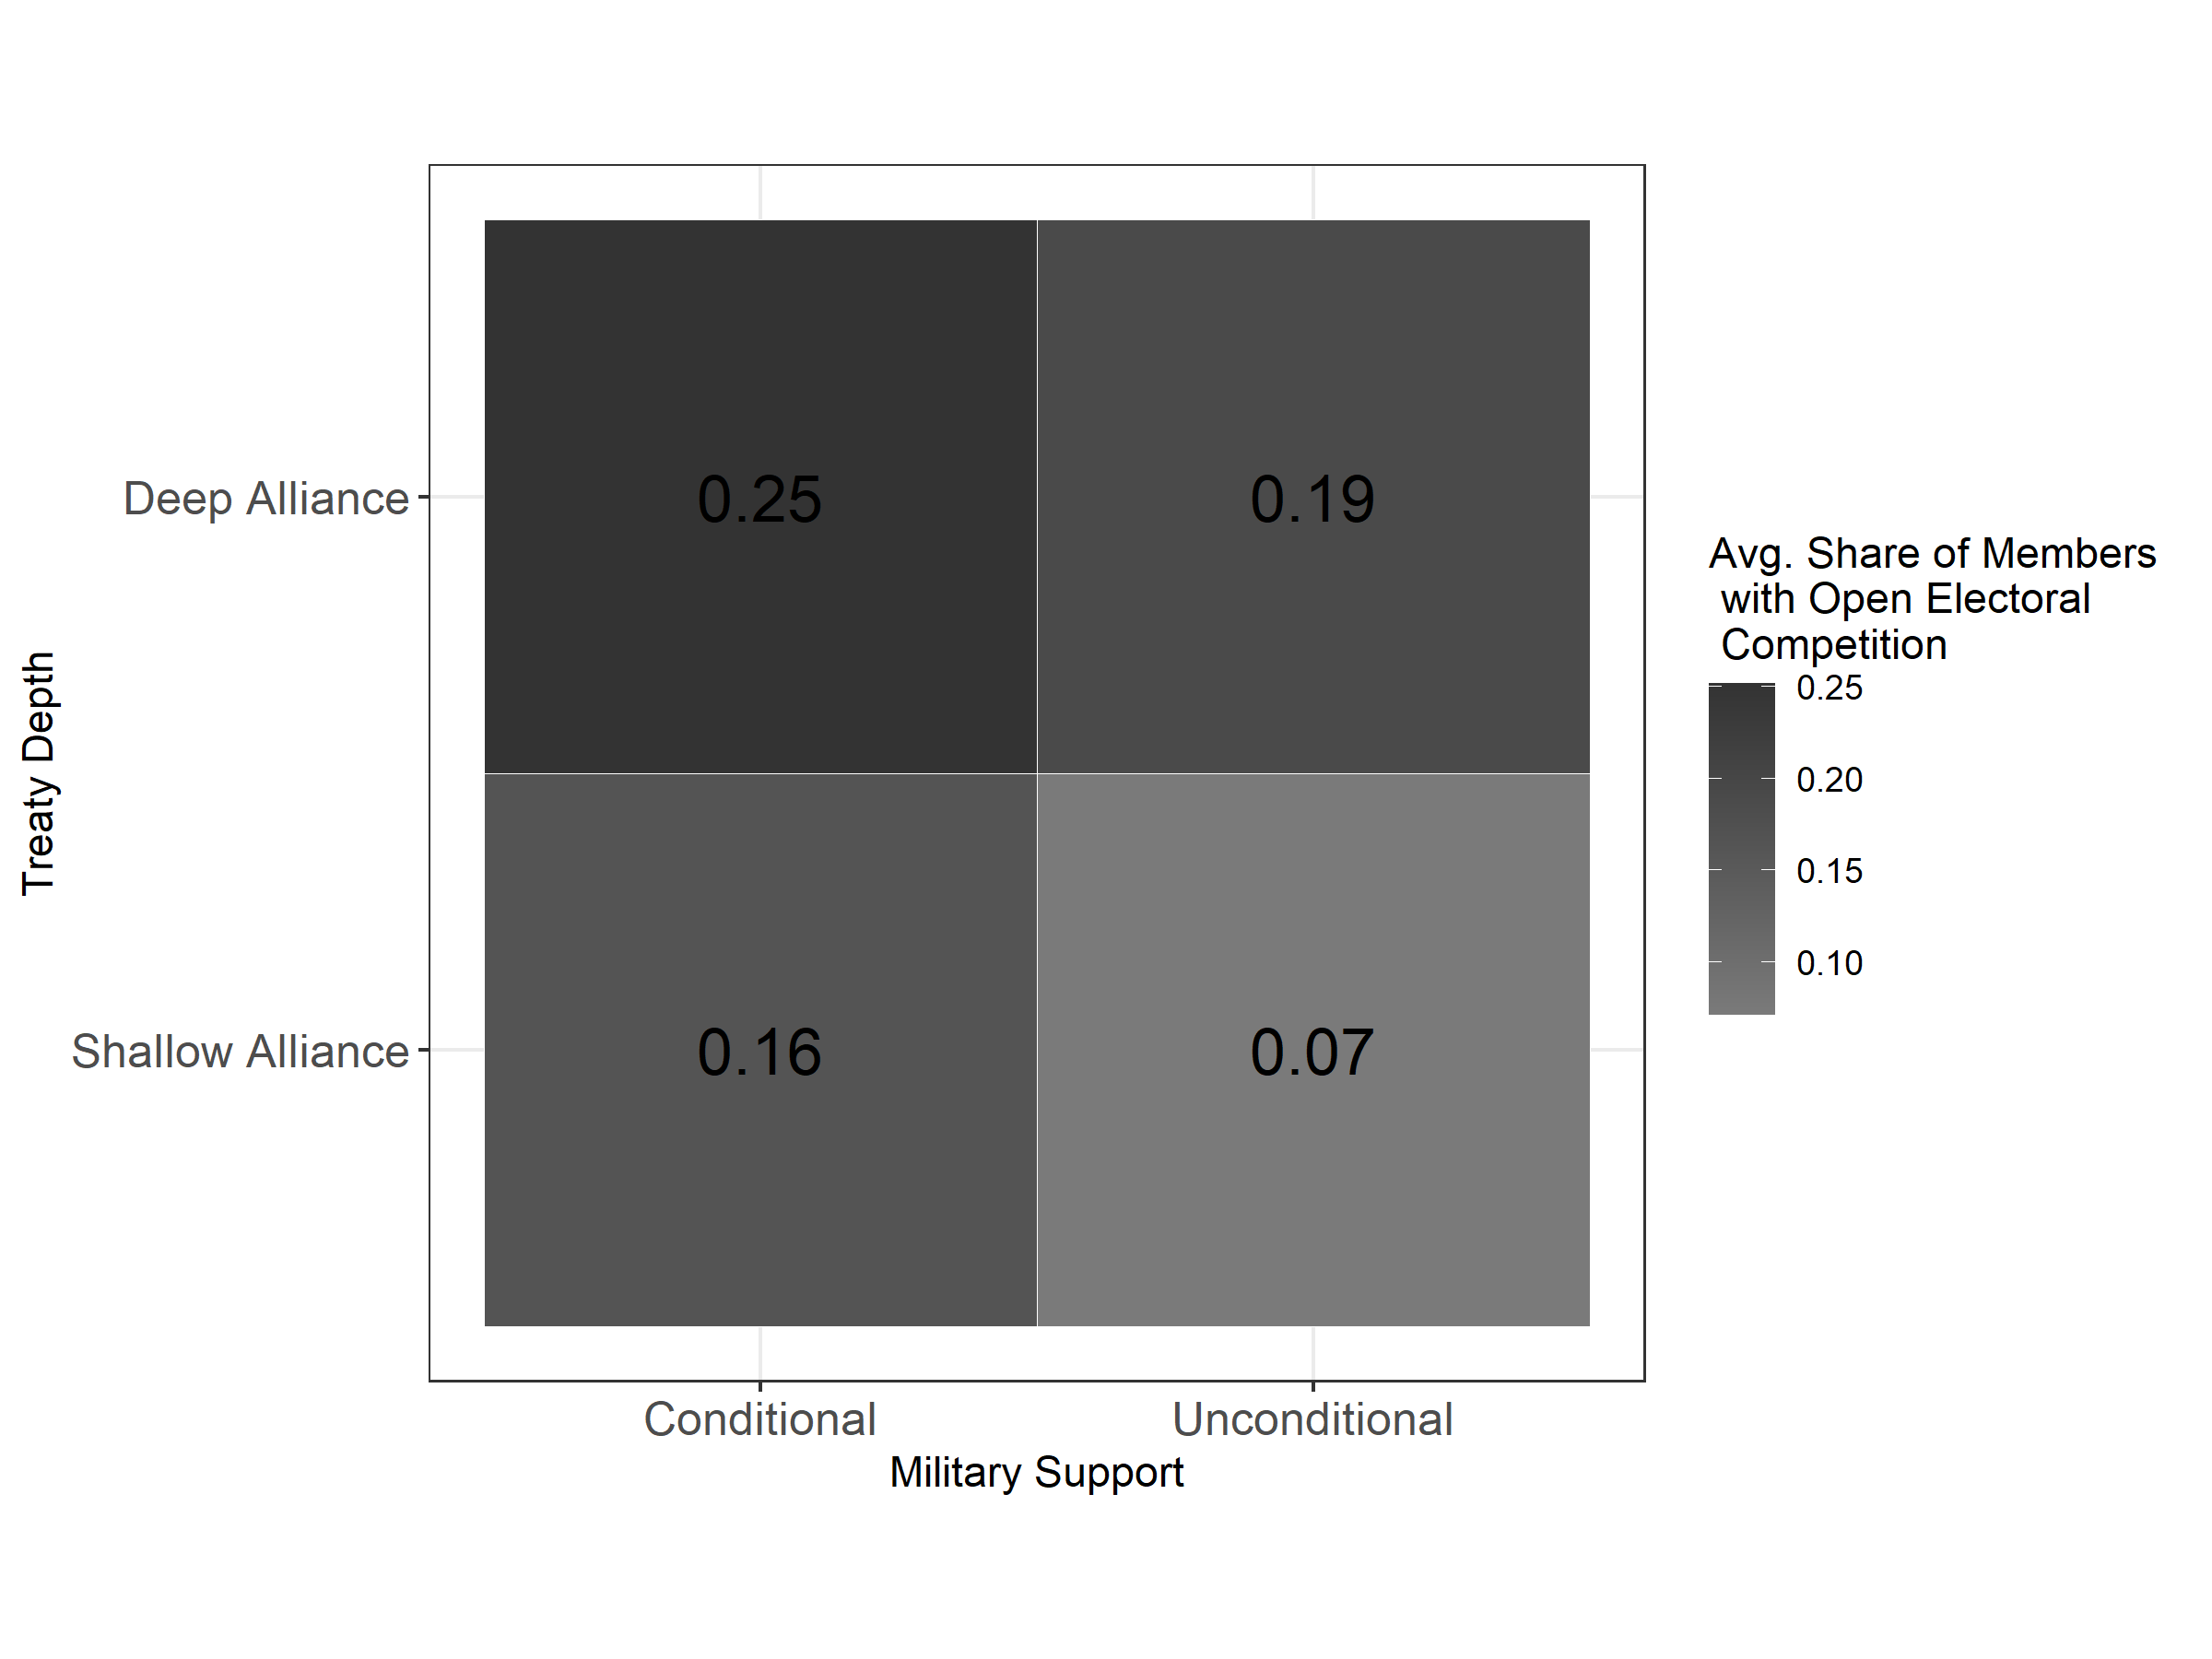
\includegraphics[width=.95\textwidth]{democ-prop-combo.png}  
\caption{Average proportion of democratic members in four groups of alliances. Alliances are grouped based on treaty depth and unconditional military support.}
\label{fig:democ-prop-combo}
\end{figure}


Results from a generalized joint regression model of treaty depth and unconditional military support match the findings in the paper.
In \autoref{fig:results-prop}, there is a no substantive association between the proportion of democracies in an alliance and the probability of unconditional military support. 
Alliances between democracies are more likely to have high treaty depth, however. 
Therefore, I find little evidence that democracies are more likely to form alliances with conditional obligations, but I do find a positive relationship between democratic alliance membership and treaty depth. 


\begin{figure}
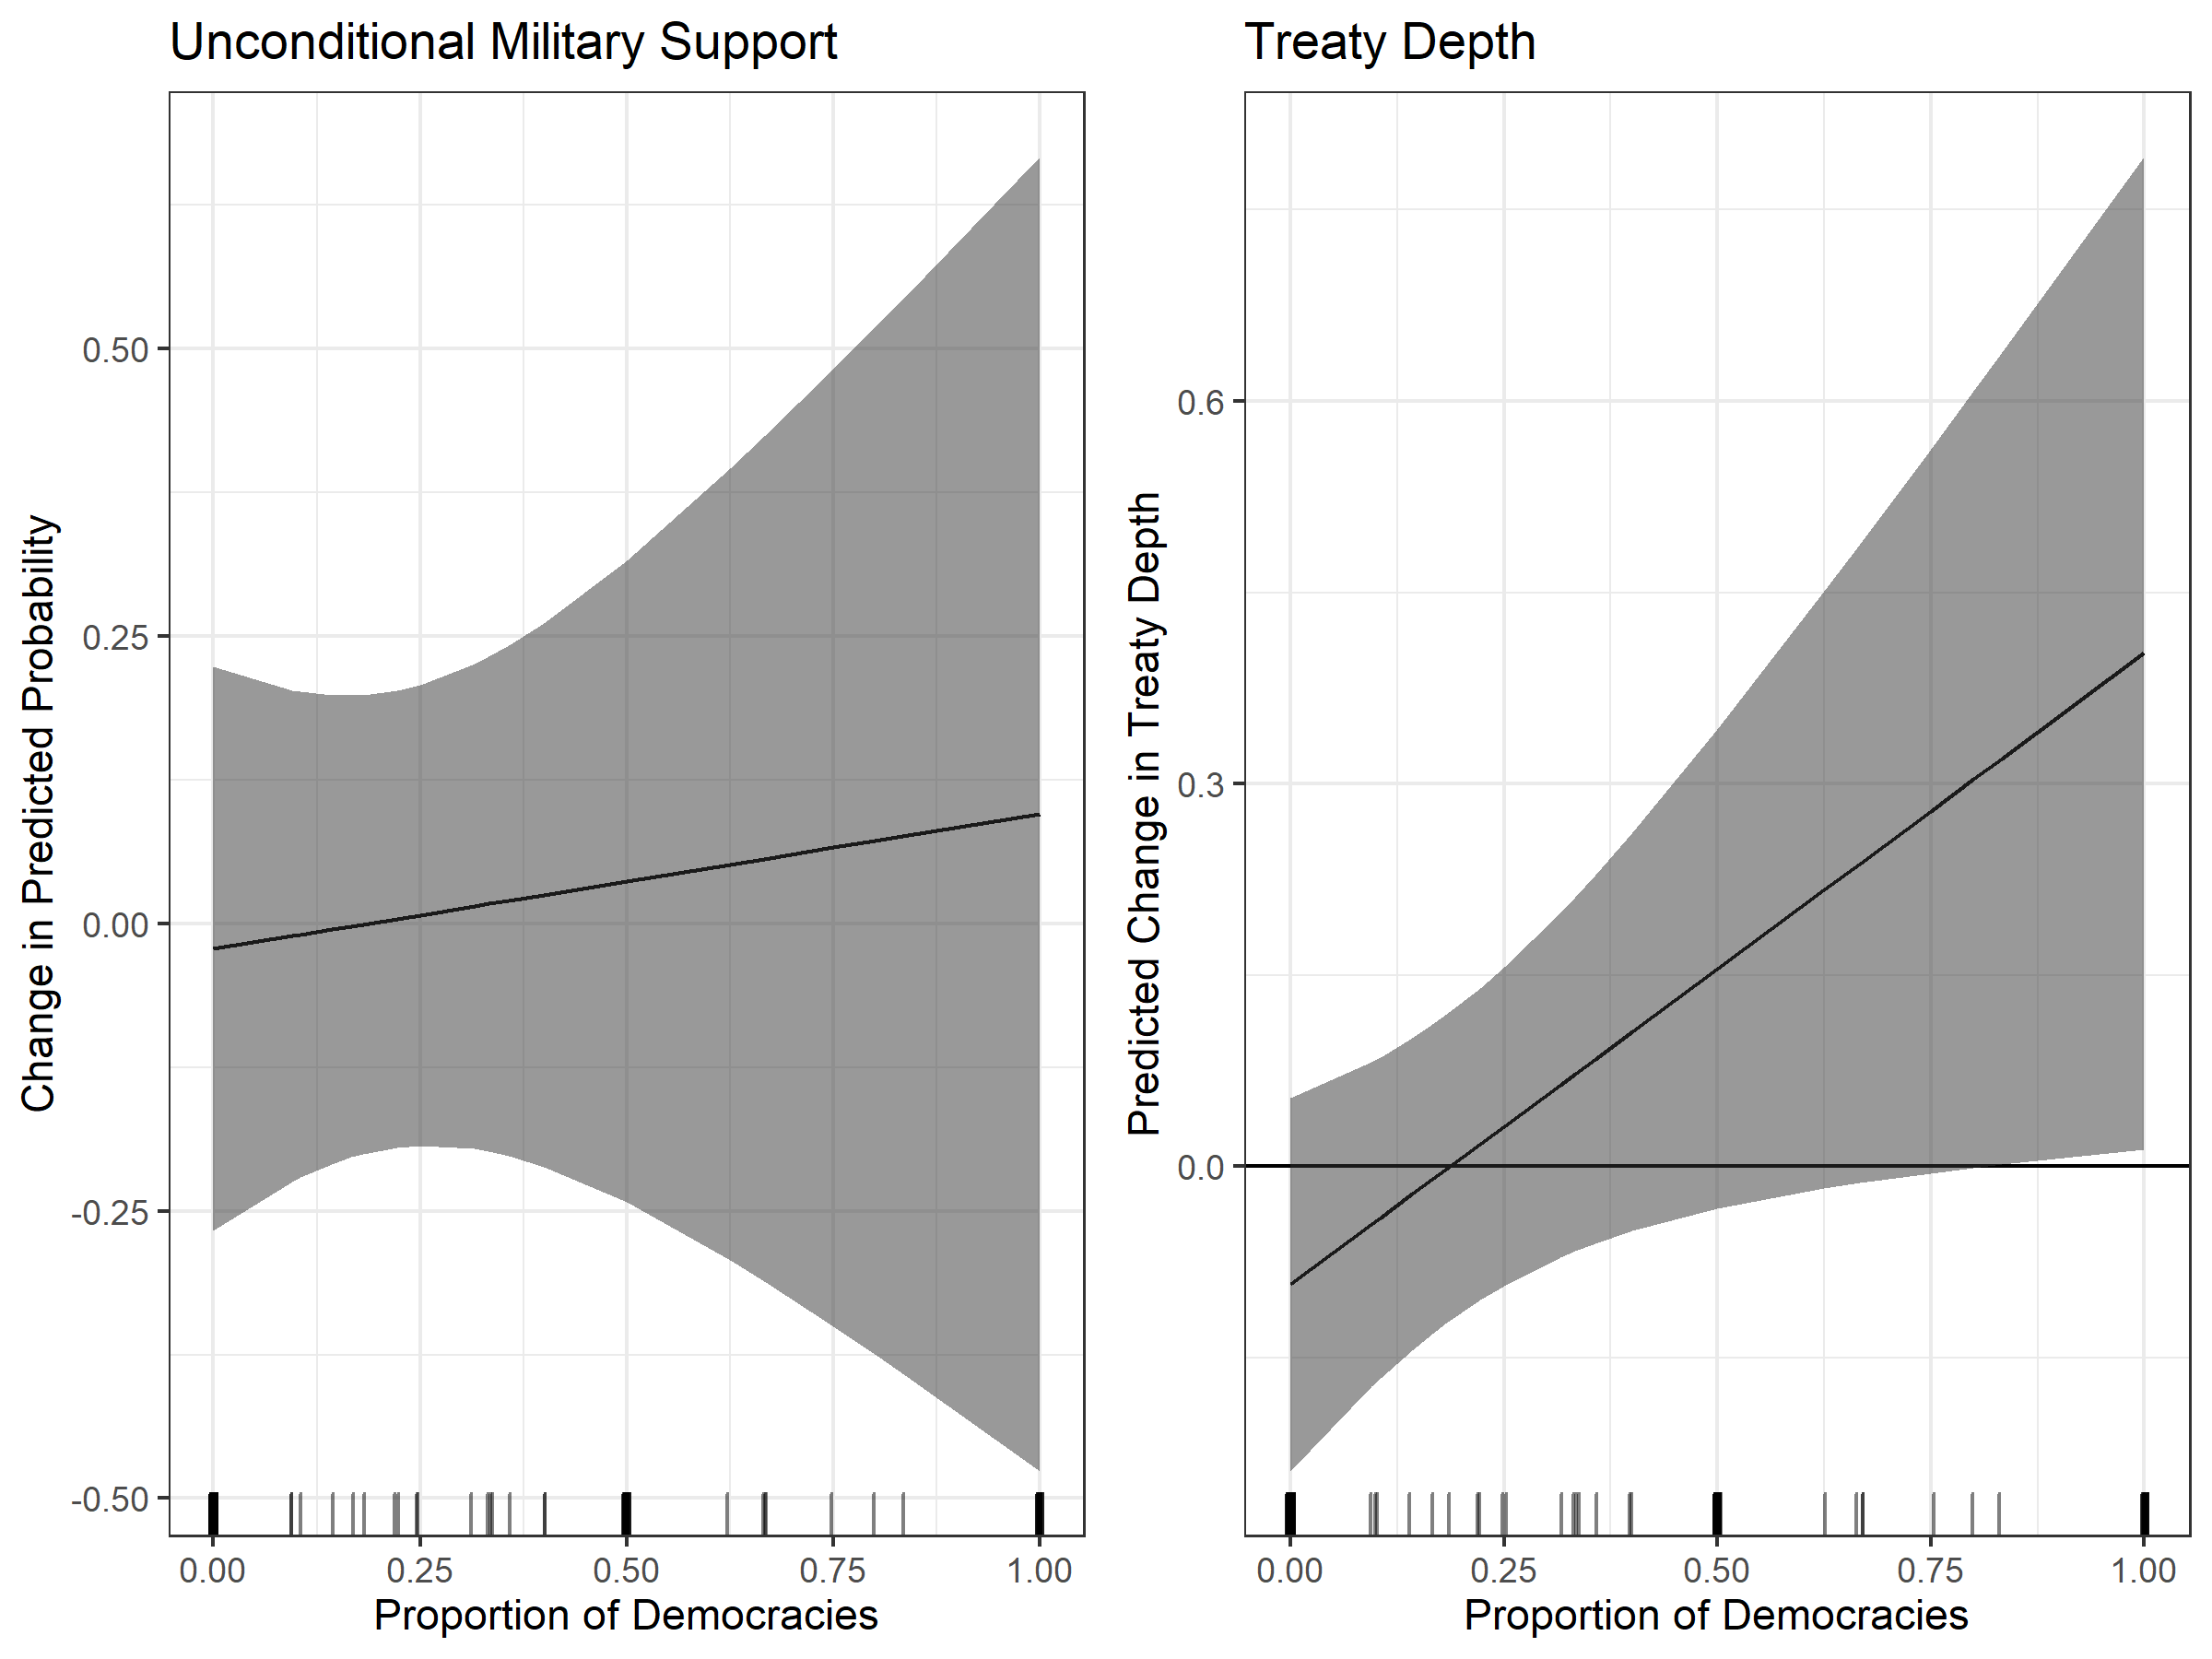
\includegraphics[width=.95\textwidth]{results-prop.png}  
\caption{Predicted probabilities of unconditional military support and predicted changes in treaty depth by the the proportion of democratic alliance members. The line marks predicted values, and the shaded areas encapsulate the standard errors. The rug plot on the x-axis marks observed values of allied democracy. Predictions based on the smoothed terms from the joint generalized regression model.}
\label{fig:results-prop}
\end{figure}





\section{Alternative Measures of Treaty Depth}


There are two measures of treaty depth that operationalize similar concepts. 
\citet{LeedsAnac2005} develop an ordinal measure of military institutionalization.
\citet{BensonClinton2016} use a latent variable model to model treaty depth. 
While my measure is a better fit for my purposes in this paper, I find somewhat similar results with these two models. 
The null finding about unconditional military support holds. 
The Leeds and Anac measure of military institutionalization produces similar results in a GRJM model. 
The Benson and Clinton measure is harder to compare, because it covers fewer alliances and has more outliers that may impact inferences.


\autoref{fig:results-alt-measures} plots predictions from the average democracy smooth term for the two alternative measures. 
For the military institutionalization measure, I could not find an ordinal model in GJRM. 
Therefore, I created a dummy variable which is equal to one if the alliance had an institutionalization score of 1 or 2. 
I then modeled the military institutionalization dummy with a probit distribution. 
The results of this analysis match the treaty depth hypothesis, as the probability of military institutionalization is increasing in average democracy. 


\begin{figure}
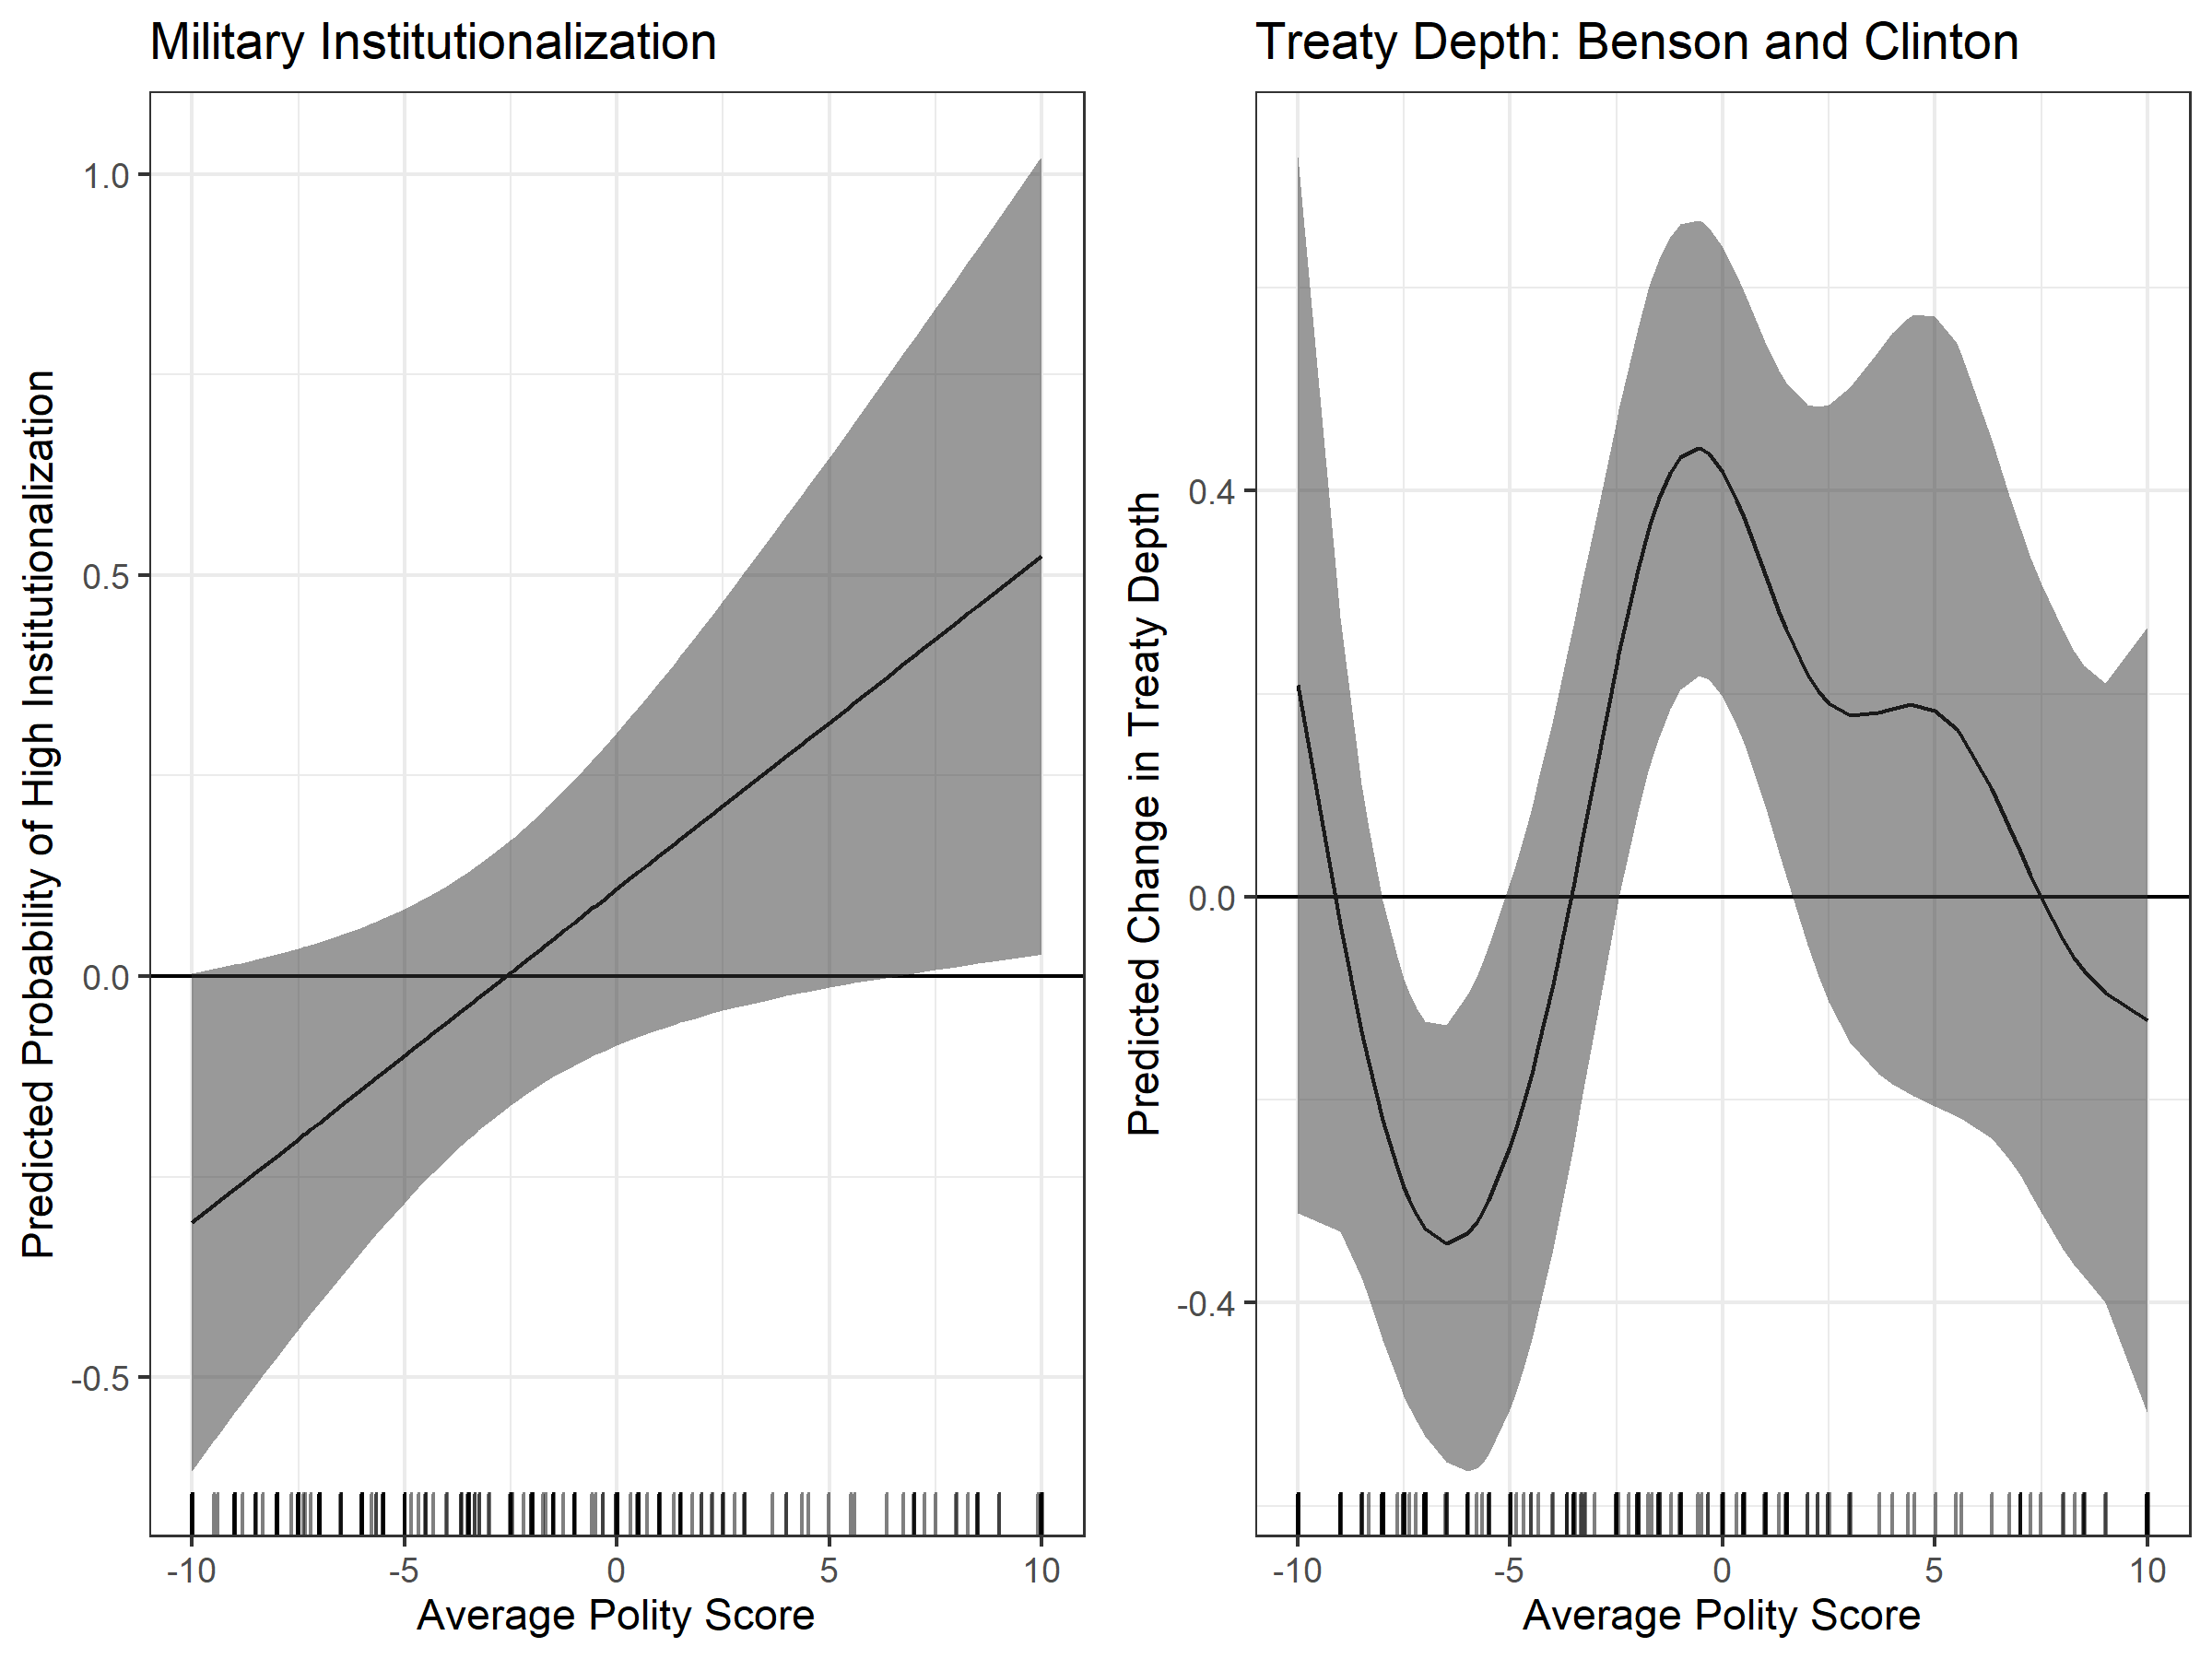
\includegraphics[width=.95\textwidth]{results-alt-measures.png}  
\caption{Predicted probabilities of unconditional military support and predicted changes in treaty depth by the the proportion of democratic alliance members. The line marks predicted values, and the shaded areas encapsulate the standard errors. The rug plot on the x-axis marks observed values of allied democracy. Predictions based on the smoothed terms from the joint generalized regression model.}
\label{fig:results-alt-measures}
\end{figure}

Findings about the association between treaty depth and Benson and Clinton's measure are more mixed. 
The relationship is highly non-linear, and high average democracy is not positively correlated with Benson and Clinton's measure of depth. 


\section{Uncertainty in Treaty Depth} 

In a separate model, I consider how measurement uncertainty shapes inferences about the connection between non-major power alliances and treaty depth. 
The latent measure of treaty depth has some uncertainty. 
This is a reasonable approximation of alliance politics, because alliance treaty depth is not observed with certainty. 
There are perceptible differences in treaty depth, especially once states add substantial depth to the treaty. 
Even so, the results from the analysis of mean treaty depth may overstate the effect of non-major power membership. 


To incorporate uncertainty over treaty depth, I fit a modification of the joint model. 
First, I created 1,000 datasets, one for each draw of the posterior distribution of the latent measure.
Then I fit the model of mean treaty depth to 500 randomly sampled datasets from those 1,000 to facilitate computation. 
For models of depth with uncertainty, I use BRMS \citep{Buerkner2017}. 
BRMS is an interface to STAN, a probabilistic programming language for Bayesian estimation \citep{Carpenteretal2016}. 
Joint Bayesian estimation has the flexibility to incorporate the probit and beta models and can be easily extended to account for uncertainty in the depth measure, but it does not allow correlated errors. 
Fitting the model sequentially to each dataset produces 500 separate models, which I combine into a single model by aggregating the posterior draws in a single posterior that accounts for uncertainty in the treaty depth measure.\footnote{Standard convergence diagnostics indicate convergence in all 500 models. Diagnostics like $\hat{r}$ are less useful for the full posterior, because some of the chains in the submodels do not overlap.}
This approach is analogous to common techniques for analyzing missing data, where multiple imputation generates uncertainty about the missing values \citep{Hollenbachetal2018imp}.
After multiple imputation, researchers fit a separate model to each imputed dataset and then combine the results. 


% Expand on these results later 
After accounting for uncertainty over treaty depth, I find a similar pattern. 
Allied democracy increases treaty depth, but decreases the probability of unconditional military support. 


\singlespace
 
\bibliography{../../../MasterBibliography} 





\end{document}